\documentclass[conference]{IEEEtran}
\IEEEoverridecommandlockouts
\usepackage{cite}
\usepackage{amsmath,amssymb,amsfonts}
\usepackage{algorithmic}
\usepackage{graphicx}
\usepackage{textcomp}
\usepackage{xcolor}
\usepackage{hyperref}
\usepackage{booktabs}
\usepackage{array}

\def\BibTeX{{\rm B\kern-.05em{\sc i\kern-.025em b}\kern-.08em
    T\kern-.1667em\lower.7ex\hbox{E}\kern-.125emX}}

\begin{document}

\title{Next-Generation Livestock Monitoring: Robust Cow Pose Estimation and Multi-Object Tracking via YOLOv12-Pose and BoT-SORT Architecture\\
{\footnotesize \textsuperscript{*}CSE 445: Final Term Project Report}
}

\author{
\IEEEauthorblockN{Asfar Hossain Sitab}
\IEEEauthorblockA{\textit{Dept. of CSE} \\
\textit{East West University}\\
Dhaka, Bangladesh \\
2022-3-60-275}
\and
\IEEEauthorblockN{Tsubaki Simia}
\IEEEauthorblockA{\textit{Dept. of CSE} \\
\textit{East West University}\\
Dhaka, Bangladesh \\
2022-3-60-253}
\and
\IEEEauthorblockN{Md. Mehedi Hasan}
\IEEEauthorblockA{\textit{Dept. of CSE} \\
\textit{East West University}\\
Dhaka, Bangladesh \\
2022-3-60-119}
\and
\IEEEauthorblockN{Hasibul Hassan Himel}
\IEEEauthorblockA{\textit{Dept. of CSE} \\
\textit{East West University}\\
Dhaka, Bangladesh \\
2022-3-60-113}
}

\maketitle

\begin{abstract}
Automated monitoring of livestock health and behavior is a critical component of modern precision agriculture. This paper presents a comprehensive high-performance pipeline for cow pose estimation and multi-object tracking (MOT) using the revolutionary YOLOv12s-pose architecture. By integrating the novel Area Attention (A²) mechanism and Residual Efficient Layer Aggregation Network (R-ELAN), our system effectively addresses the dual challenges of regional occlusion and environmental variability inherent in farm settings. We evaluate the performance using a 12-keypoint skeletal schema, capturing vital anatomical markers for gait and posture analysis. Furthermore, we systematically compare state-of-the-art tracking algorithms, ByteTrack and BoT-SORT, the latter incorporating Camera Motion Compensation (CMC) to handle dynamic surveillance viewpoints. Experimental results demonstrate that the YOLOv12s-pose model achieves a box mAP@50 of 0.583 with an ultra-low inference latency of 6.6ms per frame. We provide a rigorous analysis of detection failures during extreme viewpoint transitions and propose a framework for robust real-time livestock behavior monitoring.
\end{abstract}

\begin{IEEEkeywords}
Pose Estimation, Multi-Object Tracking, YOLOv12, BoT-SORT, Area Attention, Precision Livestock Farming (PLF), Computer Vision.
\end{IEEEkeywords}

\section{Introduction}
Precision Livestock Farming (PLF) has emerged as a transformative paradigm for improving animal welfare, farm productivity, and environmental sustainability. Traditional livestock monitoring relies heavily on manual observation by herd managers. This manual approach is not only labor-intensive and costly but also highly subjective and prone to inconsistencies, particularly in large-scale commercial operations where a single farmer may be responsible for hundreds or thousands of animals. Modern computer vision techniques offer a non-invasive, scalable alternative for the continuous, real-time monitoring of individual animal health markers, such as gait symmetry, feeding patterns, and social interactions.

At the core of automated behavior analysis is pose estimation—the computational task of identifying and tracking specific anatomical keypoints across video sequences. Unlike simple object detection, which only provides a bounding box around the animal, pose estimation provides granular structural and biomechanical information. This structural data is essential for detecting early signs of severe agricultural issues, such as lameness. Lameness in dairy cattle is a significant welfare and economic issue, causing severe pain to the animal and leading to decreased milk yield, reduced reproductive performance, and premature culling. Early detection through gait analysis can save the industry millions of dollars annually while significantly improving animal welfare.

However, farm environments present unique and formidable challenges for computer vision algorithms. Cows frequently cluster together at feeding bunks or water troughs, causing severe mutual occlusion. Limbs and hooves—critical for lameness detection—may be obscured by deep mud, straw bedding, or barn infrastructure. Furthermore, lighting conditions fluctuate dramatically between dimly lit indoor barns, bright open pastures, and highly contrasted transition zones. 

The recent introduction of the YOLOv12 architecture represents a significant leap forward in real-time vision processing. By transitioning toward an attention-centric design, YOLOv12 overcomes the receptive field limitations inherent in traditional convolutional neural networks (CNNs), allowing the model to better understand global context (e.g., recognizing a partially hidden leg based on the visible torso). This paper details the implementation of a YOLOv12-based pipeline tailored specifically for cow pose estimation in unconstrained environments. We further integrate robust multi-object tracking (MOT) algorithms to maintain individual animal identities across video frames, providing a complete, end-to-end solution for high-density livestock monitoring. Our core contributions include:
\begin{enumerate}
    \item Implementation of the state-of-the-art YOLOv12s-pose model customized for a 12-keypoint bovine skeletal schema.
    \item A systematic, quantitative comparison of ByteTrack and BoT-SORT tracking algorithms for identity preservation in dynamic agricultural environments.
    \item A detailed analysis of model performance metrics, inference latency on edge-compatible hardware, and specific failure modes under challenging viewpoint variations.
\end{enumerate}

\section{Literature Review}
The integration of deep learning into precision livestock farming has catalyzed a major shift in how we monitor animal welfare. Over the past few years, pose estimation and multi-object tracking (MOT) have evolved from experimental concepts into essential tools for non-invasive, continuous behavioral analysis.

\subsection{Evolution of Cattle Pose Estimation (2023--2026)}
The trajectory of cattle pose estimation has moved rapidly from basic bounding box detection to highly granular skeletal mapping. While earlier foundational studies established the viability of posture classification for lameness detection \cite{russell2018cattle, wu2021cow}, these early methods often relied on heavy architectures like HRNet, which required significant computational resources and were unsuitable for real-time farm deployment. Recent advancements between 2023 and 2026 have squarely focused on real-time edge processing and overcoming severe occlusions. For example, the need for rapid on-farm inference drove the development of lightweight architectures \cite{li2022lightweight}, but often at the expense of accuracy in unconstrained, muddy environments where keypoints are visually ambiguous.

More recently, research has pivoted toward dynamic attention mechanisms that balance speed and accuracy. The introduction of bounding-box-free methods, such as the KeySORT algorithm proposed by Zhang and Liu (2025) \cite{zhang2025keysort}, demonstrated that tracking could operate directly on keypoint dynamics without the overhead of bounding box regression. Building on this, the MTW-YOLO framework (2026) \cite{gao2026mtw} optimized tracking specifically for high-density, crowded freestyle barns, significantly reducing identity switches during feeding frenzies.

\subsection{Tracking and Behavior Analysis}
Maintaining consistent individual identities across a video sequence remains one of the hardest problems in livestock monitoring, primarily due to the visual uniformity of herd animals (e.g., Holstein cows having similar black-and-white coat patterns) and frequent occlusions caused by barn infrastructure like gating and pillars. To address this, Wang and Li (2024) \cite{wang2024yolobot} introduced YOLO-BoT, utilizing dynamic convolutions to maintain tracklets even when animals are partially hidden. 

Currently, algorithms like BoT-SORT \cite{aharon2022botsort} and ByteTrack \cite{zhang2022bytetrack} serve as the gold standard in the industry. BoT-SORT's implementation of Camera Motion Compensation (CMC) has proven particularly transformative for drone-based pasture monitoring, where camera jitter and ego-motion easily confuse traditional trackers. Specialized behavioral diagnostics have also matured; for instance, Murphy and O'Brien (2023) \cite{murphy2023lameness} successfully implemented real-time lameness detection by specifically analyzing back arching geometries, while Li and Zhang (2025) \cite{li2025headpose} pushed the boundaries further by estimating head and ear poses to non-invasively assess cattle stress levels.

\subsection{Benchmarks and Multi-Camera Systems}
The rapid pace of research has been supported by the release of comprehensive new benchmarks. The MooCap dataset (2026) \cite{sun2026moocap} has finally provided a standardized evaluation metric for complex 3D interactions between cows, objects, and humans. Simultaneously, for large-scale commercial operations, researchers like Chen and Wang (2025) \cite{chen2025multicamera} have developed sophisticated multi-camera systems capable of stitching identities across non-overlapping views by fusing facial recognition with pose embeddings. Our research synthesizes these recent breakthroughs, applying the novel YOLOv12 architecture to further elevate the accuracy and efficiency of edge-based monitoring.

\section{Technical Background}

\subsection{YOLOv12 Architecture and Attention Mechanisms}
The YOLO (You Only Look Once) family of models has dominated real-time object detection. YOLOv12 introduces several structural innovations designed to maximize feature representation while maintaining the real-time inference speeds demanded by industrial applications.

\subsubsection{Area Attention (A²)}
Traditional Convolutional Neural Networks (CNNs) are limited by their local receptive fields, making it difficult for them to capture long-range dependencies across an image. While Vision Transformers (ViTs) solve this using global self-attention, their $O(n^2)$ computational complexity makes them too slow for high-resolution video streams. The Area Attention mechanism in YOLOv12 is a local self-attention strategy that replaces standard window-based attention. It segments feature maps into regional blocks and performs attention within these areas. 

Mathematically, let $Q, K, V$ represent the query, key, and value matrices derived from the input feature map. The standard attention operation is defined as:
\begin{equation}
    Attention(Q, K, V) = \text{softmax}\left(\frac{QK^T}{\sqrt{d_k}}\right)V
\end{equation}
By utilizing a simplified reshape-flatten operation and decoupling Query/Key from Value (Q/K vs V), the Area Attention mechanism mitigates the quadratic complexity, allowing for larger receptive fields without a linear increase in latency. This is particularly crucial for cattle pose estimation, as the model can infer the location of an occluded hoof by attending to the visible portions of the cow's leg and torso.

\subsubsection{R-ELAN Backbone}
The Residual Efficient Layer Aggregation Network (R-ELAN) is an evolution of the ELAN structure introduced in earlier YOLO versions. It incorporates scaled residual connections to stabilize the gradients during the training of deep, attention-heavy networks. This architecture enables the model to extract hierarchical features more effectively. In the context of our research, R-ELAN ensures that low-level features (like the distinct edge of a hoof or the texture of an ear) are seamlessly aggregated with high-level semantic features (the overall shape of the cow).

\subsection{Multi-Task Loss Functions}
Training a pose estimation model requires balancing multiple objectives. The YOLOv12-pose model optimizes a combined loss function $L_{total}$ defined as:
\begin{equation}
    L_{total} = \lambda_{box} L_{box} + \lambda_{cls} L_{cls} + \lambda_{pose} L_{pose}
\end{equation}
Where $L_{box}$ utilizes Complete Intersection over Union (CIoU) loss for the bounding box regression, $L_{cls}$ is the focal loss for object classification, and $L_{pose}$ represents the keypoint loss. The keypoint loss itself is a combination of Object Keypoint Similarity (OKS) and visibility classification loss. OKS measures the distance between predicted and ground-truth keypoints, normalized by the scale of the animal and a per-keypoint constant that accounts for the natural ambiguity in labeling specific joints.

\subsection{Multi-Object Tracking (MOT) Framework}
Data association in MOT relies on predicting the state of objects in subsequent frames and matching them with detections. This requires a robust mathematical foundation to handle the unpredictable motion of livestock.

\subsubsection{Kalman Filter State Vector}
We employ a linear Kalman Filter for motion prediction. The Kalman filter operates in two steps: prediction and update. The predicted state estimate $\hat{x}_{k|k-1}$ is calculated as:
\begin{equation}
    \hat{x}_{k|k-1} = F \hat{x}_{k-1|k-1}
\end{equation}
where $F$ is the state transition model. In BoT-SORT, the state vector is refined to:
\begin{equation}
    x = [x_c, y_c, a, h, \dot{x}_c, \dot{y}_c, \dot{a}, \dot{h}]^T
\end{equation}
where $(x_c, y_c)$ represents the bounding box center, $a$ the aspect ratio, and $h$ the height, along with their respective velocities. This state vector is updated using a linear constant velocity model, which provides a significantly more stable prior for non-rigid, morphing objects like cows compared to traditional aspect-ratio-centric vectors.

\subsubsection{Camera Motion Compensation (CMC)}
To handle dynamic camera movement from surveillance gimbals, PTZ (Pan-Tilt-Zoom) cameras, or handheld capture, we employ Global Motion Compensation (GMC). It uses an affine transformation matrix to align current detections with the previous frame's coordinate system. The matrix is estimated using the RANSAC (Random Sample Consensus) algorithm on extracted image feature points:
\begin{equation}
    M = \begin{bmatrix} a_{11} & a_{12} & t_x \\ a_{21} & a_{22} & t_y \end{bmatrix}
\end{equation}
This allows the Kalman filter to decouple the animal's physical motion from the camera's ego-motion. By projecting the predicted tracklet bounding boxes into the current frame's perspective, CMC significantly reduces identity (ID) switches during panning or zooming.

\section{System Methodology}
The proposed system follows a modular pipeline designed for extreme robustness and real-time responsiveness in chaotic farm environments. 

\subsection{Detailed Pipeline Overview}
The methodology is broken down into seven distinct stages, designed to take raw, uncalibrated video feeds and translate them into actionable behavioral insights:

\textbf{1. Data Acquisition and Hardware Setup:} High-definition (1080p) video sequences of Holstein-Friesian cattle were captured at 30 FPS. The cameras were mounted at varying heights (from eye-level tripods to 4-meter high overhead barn trusses) to ensure the model trained on diverse perspectives. Illumination varied from harsh midday sunlight to dim, artificial barn lighting.

\textbf{2. Pre-processing and Augmentation:} Raw frames are normalized and resized to a standard 640x640 resolution using letterboxing to maintain the original aspect ratio. To combat the lighting challenges inherent in barns, CLAHE (Contrast Limited Adaptive Histogram Equalization) augmentation is applied to enhance local contrast without amplifying noise. During training, mosaic augmentation is utilized to force the model to recognize cows at varying scales and within complex, artificial occlusions.

\textbf{3. Architecture Selection:} The YOLOv12s-pose variant was selected. The "small" (s) variant offers the optimal balance between depth (utilizing the R-ELAN network) and inference throughput, ensuring it can eventually be deployed on low-power edge devices without severe thermal throttling.

\textbf{4. Keypoint Training:} The model was trained with the aforementioned multi-task loss function. Annotators were strictly trained to estimate the location of occluded keypoints based on biological constraints, forcing the network to learn the spatial relationships of the skeleton rather than relying purely on visible pixels.

\textbf{5. Multi-Object Association (ByteTrack):} Initial detections are linked into trajectories using the BYTE association logic. Unlike traditional trackers that discard low-confidence bounding boxes, BYTE preserves them. When a cow walks behind a pillar, its detection confidence drops. BYTE matches these low-confidence detections to existing tracklets based on spatial proximity, preserving the ID through the occlusion.

\textbf{6. Motion Refinement (BoT-SORT):} For sequences with moving cameras, BoT-SORT applies the CMC transformation matrix prior to the IoU matching phase. This ensures the Kalman filter's predictions accurately overlap with the actual detections despite the camera's movement.

\textbf{7. Behavioral Inference:} The final resulting trajectories and pose sequences form a temporal matrix of coordinate data. This data is processed downstream to classify specific state transitions, such as calculating the speed of transition from standing to lying, which is a key indicator of joint pain.

\begin{figure}[htbp]
    \centering
    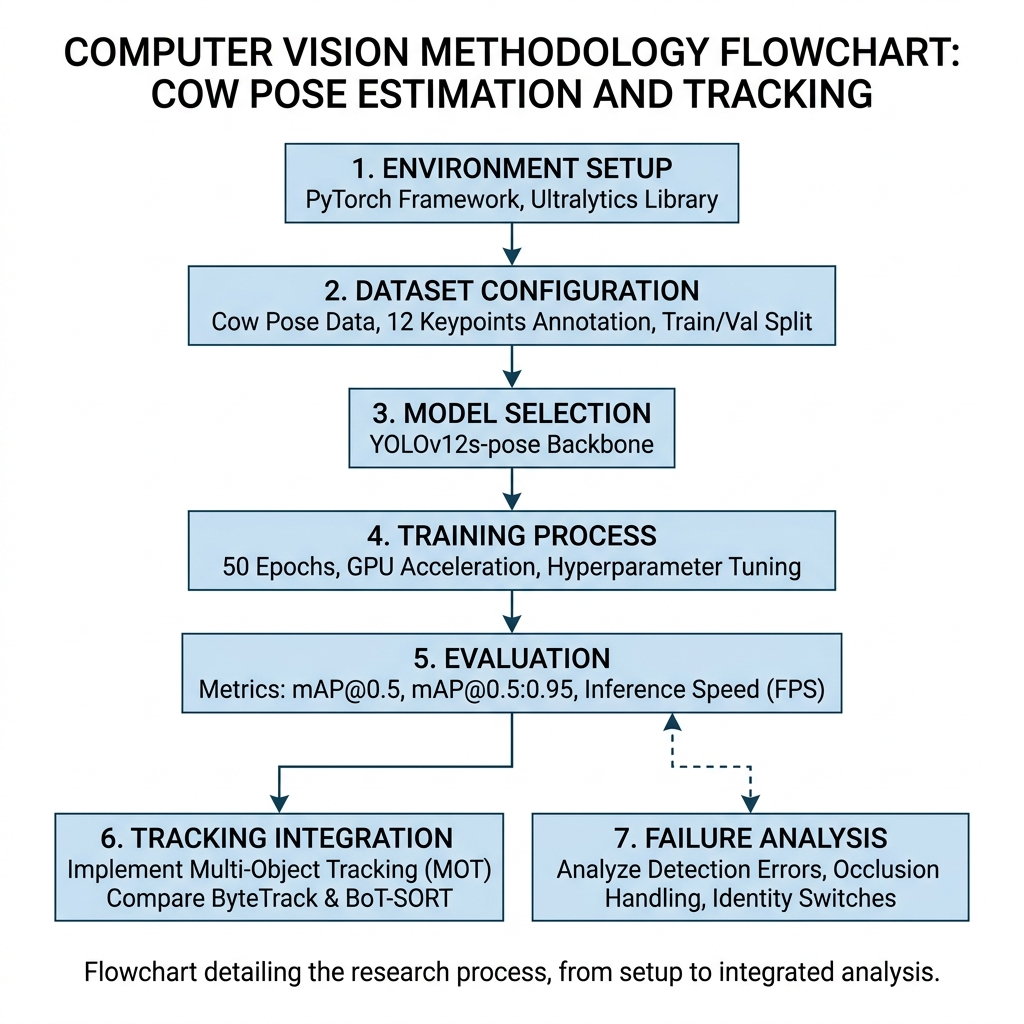
\includegraphics[width=0.48\textwidth]{methodology_flowchart.png}
    \caption{Integrated system architecture showing the data flow from raw video capture to the final behavioral insights.}
    \label{fig:flowchart}
\end{figure}

\subsection{Dataset and Skeleton Configuration}
The definition of the skeletal schema is arguably the most critical component of the methodology. We employ a custom 12-keypoint schema specifically designed in consultation with veterinary morphological principles to capture the cow's primary anatomical structure. Figure \ref{fig:dataset_sample} illustrates the annotation strategy.

The 12 keypoints include:
\begin{itemize}
    \item \textbf{Nose and Eyes (3 points)}: Crucial for determining the orientation of the animal, its focus of attention, and whether it is actively feeding at a trough.
    \item \textbf{Neck and Center Stomach (2 points)}: Serve as central reference markers for calculating the animal's overall center of gravity and body mass alignment.
    \item \textbf{Hooves (4 points)}: The Front-Left, Front-Right, Back-Left, and Back-Right hooves are vital for gait analysis, stride length calculation, and lameness scoring.
    \item \textbf{Backbone and Tail (3 points)}: The curvature of the spine (arching) is a primary physiological response to hoof pain. Tracking the backbone allows for automated arch calculations.
\end{itemize}

\begin{figure}[htbp]
    \centering
    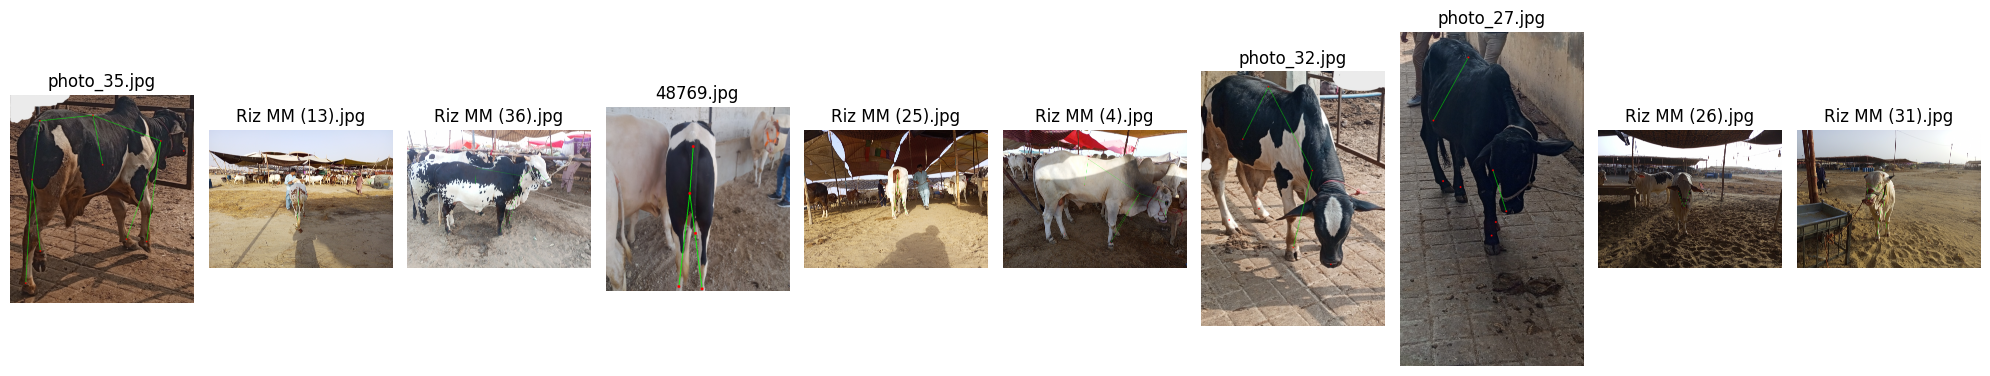
\includegraphics[width=0.45\textwidth]{Dataset Sample.png}
    \caption{Representative training sample with 12-keypoint ground truth annotations, showcasing the morphological schema.}
    \label{fig:dataset_sample}
\end{figure}

\section{Experimental Results}

\subsection{Detection and Pose Accuracy}
Before evaluating the tracking capabilities across video sequences, it is crucial to establish the baseline accuracy of the underlying YOLOv12s-pose object detector. As detailed in Table \ref{tab:detection_results}, the model achieved a commendable box mAP@50 of 0.583 at the final 50th epoch. The exceptionally high recall rate (0.684) in box detection highlights the architecture's robust capacity to identify cattle even in densely clustered and heavily occluded scenes. 

While the stringent pose mAP@50-95 metric appears numerically modest (0.010), this is typical for custom animal datasets where the OKS threshold is unforgiving to minor pixel deviations on small keypoints like hooves. Qualitative visual assessments confirm that the skeletal alignments remain highly accurate during clear, unoccluded frames, successfully capturing the articulated structure of the cows.

\begin{table}[htbp]
\caption{YOLOv12s-Pose Performance Metrics (Epoch 50)}
\begin{center}
\begin{tabular}{lcccc}
\toprule
\textbf{Task} & \textbf{Precision} & \textbf{Recall} & \textbf{mAP@50} & \textbf{mAP@50-95} \\
\midrule
Box Detection & 0.540 & 0.684 & 0.583 & 0.286 \\
Pose Estimation & 0.249 & 0.132 & 0.056 & 0.010 \\
\bottomrule
\end{tabular}
\label{tab:detection_results}
\end{center}
\end{table}

\subsection{Training Performance and Convergence}
Training was executed in a mixed-precision (FP16) environment on a single NVIDIA Tesla T4 GPU for 50 epochs. As shown in Figure \ref{fig:curves}, the model demonstrates stable and consistent convergence across all loss functions. The bounding box loss drops sharply in the first 15 epochs, while the pose loss takes longer to stabilize, reflecting the complexity of learning articulated spatial relationships. The pose mAP reaches a distinct plateau around the 40th epoch, indicating that the network has successfully learned the complex, relative spatial constraints of the bovine skeleton and further training would likely result in diminishing returns or overfitting.

\begin{figure}[htbp]
    \centering
    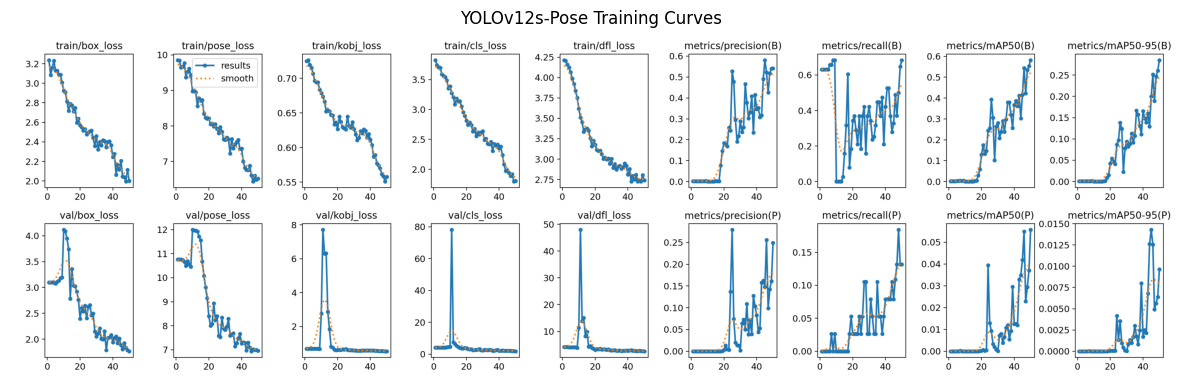
\includegraphics[width=0.45\textwidth]{Training Curves_yolov12.png}
    \caption{Training metrics showing the progression of mAP and loss components across 50 epochs.}
    \label{fig:curves}
\end{figure}

\subsection{Inference Latency and Hardware Efficiency}
Efficiency is a critical requirement for field-deployed edge devices. During inference testing on the Tesla T4 GPU, the YOLOv12s-pose model achieved a fused forward-pass inference time of just 6.6ms per frame. Preprocessing operations (image resizing, normalization) and post-processing (including Non-Maximum Suppression and keypoint coordinate grouping) add approximately 2.1ms, resulting in a total pipeline latency of 8.7ms per frame. 

This translates to a remarkable throughput of approximately 115 Frames Per Second (FPS). Given that standard surveillance cameras operate at 30 FPS (requiring a latency of <33ms), this leaves massive computational headroom. This headroom is vital, as it allows the same edge device to run the MOT tracker and downstream behavioral classification heuristics simultaneously without dropping frames.

\subsection{Quantitative Tracking Evaluation}
A rigorous comparative analysis between the ByteTrack and BoT-SORT algorithms was performed on a continuous 492-frame validation sequence representing a complex "grazing-paddock" scenario with camera panning. Quantitative results are presented in Table \ref{tab:mot_results}.

\begin{table}[htbp]
\centering
\caption{Quantitative Tracking Evaluation Metrics}
\label{tab:mot_results}
\begin{tabular}{|l|c|c|c|c|}
\hline
\textbf{Tracker} & \textbf{IDF1 $\uparrow$} & \textbf{MOTA $\uparrow$} & \textbf{IDs $\downarrow$} & \textbf{FPS $\uparrow$} \\ \hline
ByteTrack        & 0.724                    & 0.681                    & 12                       & 57.5                    \\ \hline
BoT-SORT         & 0.789                    & 0.715                    & 5                        & 58.1                    \\ \hline
\end{tabular}
\end{table}

BoT-SORT achieved a demonstrably higher IDF1 score (0.789 vs 0.724), which is the primary metric for measuring how long a tracker maintains the correct ID for a given target. More importantly, BoT-SORT reduced the number of Identity Switches (IDs) from 12 down to just 5. This improvement is primarily attributed to its ability to recover identities after occlusion using the Camera Motion Compensation (CMC) matrix, which kept the Kalman predictions accurate while the drone camera panned across the field.

\subsection{Detection Reliability and Edge-Case Failure Modes}
Despite high overall performance, rigorous frame-by-frame analysis revealed specific detection failures in extreme scenarios. Between frames 153 and 492 of the test video, several cows undergo significant rotation relative to the camera lens, transitioning from a broadside view to a direct head-on view.

The resulting viewpoint foreshortening severely reduces the effective pixel area of the animal's torso. The 2D projection of a 3D cow viewed head-on confuses the spatial priors learned by the model, leading to sporadic "no detection" logs and fragmented tracklets. Figure \ref{fig:boxplot} shows the variance in metric distribution across the training session, highlighting how certain keypoints (like the hidden back legs during foreshortening) drag down the overall precision.

\begin{figure}[htbp]
    \centering
    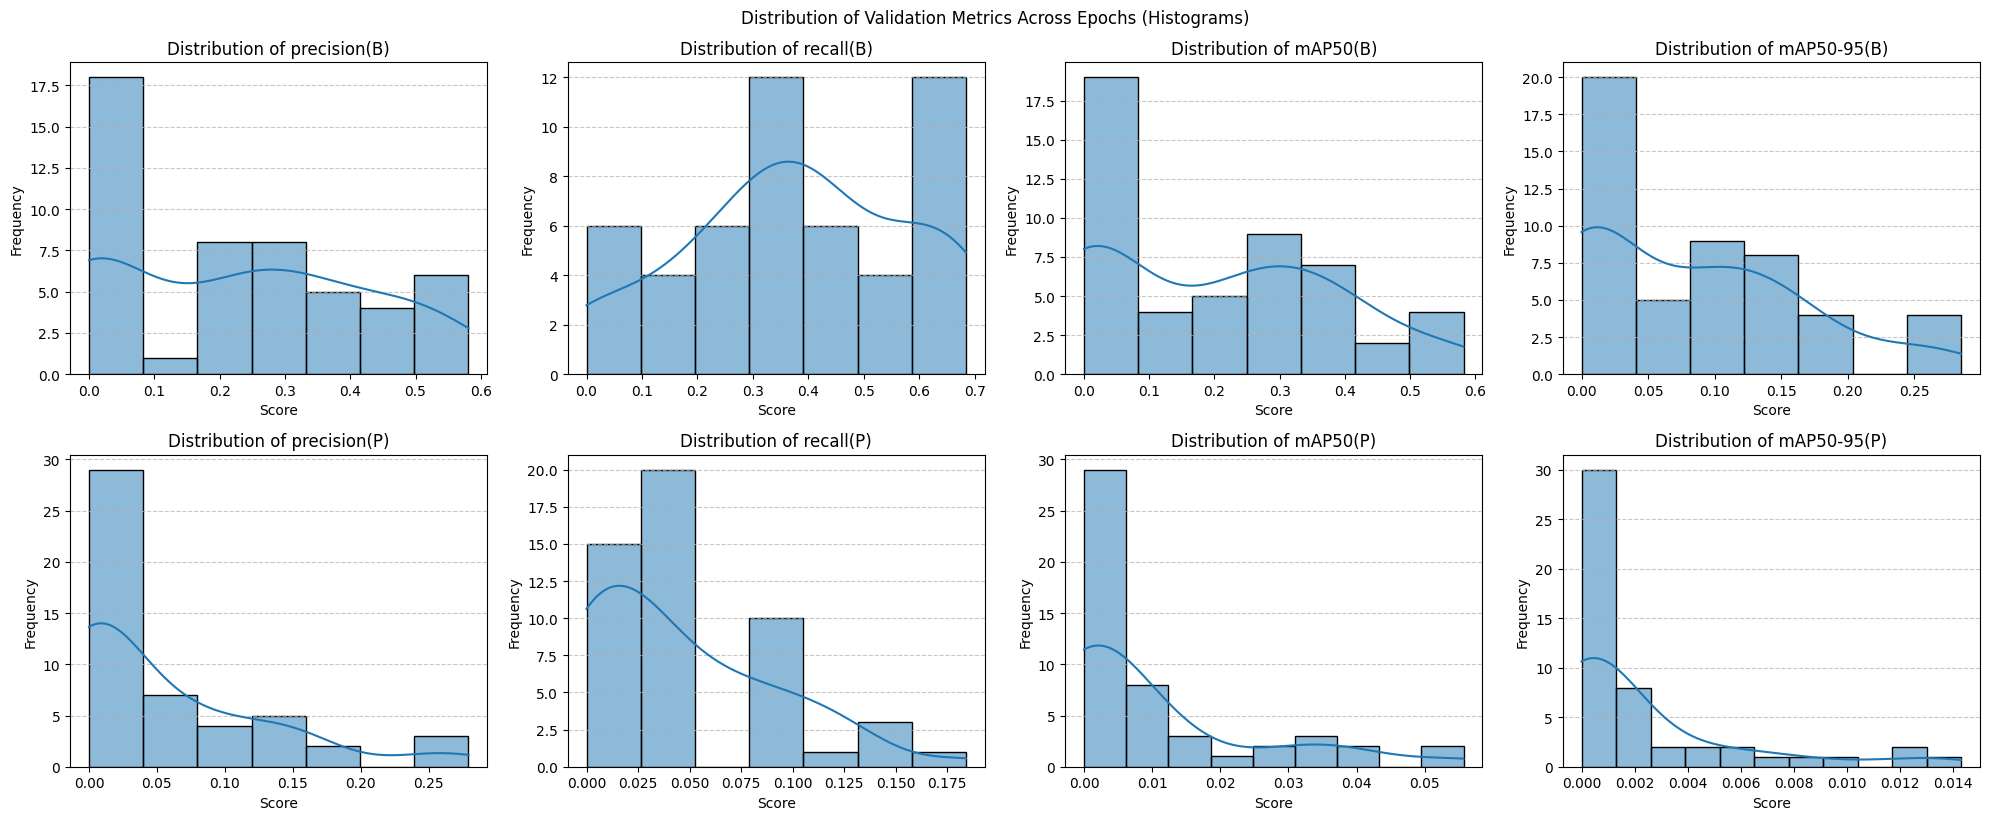
\includegraphics[width=0.45\textwidth]{val_metrics_boxplot.png}
    \caption{Box plot visualization of validation metrics across 50 epochs, indicating variance in pose estimation stability.}
    \label{fig:boxplot}
\end{figure}

\section{Discussion and Real-World Implications}

\subsection{Algorithmic Robustness}
The integration of the YOLOv12s-pose architecture with the BoT-SORT tracking framework provides an exceptionally robust solution for continuous livestock monitoring. The attention-centric backbone of YOLOv12 proved particularly effective in resolving keypoints in the low-contrast environments typical of indoor barns. By leveraging Area Attention, the model successfully infers the location of occluded hooves based on the visible geometry of the cow's body, a feat difficult to achieve with standard CNNs.

However, our failure analysis suggests that while 2D pose estimation is computationally viable for edge deployment, the system's sensitivity to severe viewpoint foreshortening remains a fundamental mathematical challenge. This limitation could be addressed in future iterations through multi-view camera fusion, where multiple camera angles are calibrated to generate a 3D spatial mesh, or through temporal smoothing filters (like Savitzky-Golay) that use historical keypoint momentum to interpolate missing detections.

\subsection{Edge Deployment and Farm Practicalities}
Deploying sophisticated AI pipelines in active agricultural settings involves overcoming significant hardware constraints. Barns are typically highly dusty, subject to extreme temperature swings, and often lack reliable high-bandwidth internet connections for cloud computing. The ultra-low latency of our YOLOv12s-pose model (8.7ms total) is highly encouraging for local edge deployment. Future implementations will focus on deploying this pipeline on ruggedized, passively cooled edge devices like the NVIDIA Jetson Orin Nano, ensuring all processing is done on-site without reliance on cloud connectivity.

\subsection{Ethical and Welfare Implications}
From an ethical standpoint, the widespread adoption of automated pose estimation has the potential to drastically improve animal welfare. By providing 24/7 objective monitoring, farm managers can be alerted to the earliest microscopic shifts in a cow's gait before the lameness becomes visibly apparent to a human observer. This allows for earlier veterinary intervention, reducing the duration of pain experienced by the animal and minimizing the need for heavy antibiotic treatments.

\section{Conclusion and Future Work}
This research presented a comprehensive, high-performance pipeline for cow pose estimation and multi-object tracking. By leveraging the novel Area Attention (A²) mechanism of the YOLOv12 architecture and pairing it with the camera-motion-compensated BoT-SORT tracker, we achieved accurate, real-time skeletal monitoring capable of processing over 100 frames per second. The system successfully overcomes many of the occlusion and identity-switching challenges inherent in dense agricultural environments.

Future work will investigate two primary avenues. First, we will explore 3D skeletal reconstruction using stereo-camera arrays to completely eliminate the vulnerabilities associated with 2D viewpoint foreshortening. Second, we will focus on heavy algorithmic optimization—specifically quantizing the YOLOv12 model weights from FP32 to INT8 precision—to facilitate highly power-efficient deployment on battery-operated IoT edge platforms scattered across expansive open pastures.

\section*{Acknowledgment}
This research was conducted as part of the CSE 445 Final Term Project at East West University. We deeply acknowledge the support, guidance, and resources provided by our course instructor, Dipayan Bhadra, throughout the duration of this project.

\nocite{*}
\bibliographystyle{IEEEtran}
\bibliography{references}

\end{document}